% \lipsum[2-4]

VR is also being studied by aeronautics and aerospace industries. \citeauthor{moerland2021application} proposed the use of the VR during the aircraft cabin's design procedure. The idea is to create a easy communication between the development actors and it's clients.

The cabin design procedure is often said to be a complex product because it involves a lot of users and stakeholder and each of them have their own set of preferences and requirements \citeauthor{moerland2021application}. The time needed to attend all of these demands tend to be long and expensive. In order to understand better the design process of an aircraft cabin, \citeauthor{moerland2021application} interviewed an cabin designer and the conclusion of this interview was that the cabin design needed in general 2 years to be concluded. As an example, the interviewed cited a design that multiples mock-ups and more than ten meetings with the stakeholder were needed while designing the cabin. The Figure \ref{fig:simplified_cabin_process} illustrates a simplified cabin design process and shows that the traditional process has a high chance to return to initials phases even at final phases.

%\begin{figure}[h]
%\centering
%\begin{minipage}{\textwidth}
%    \centering
%    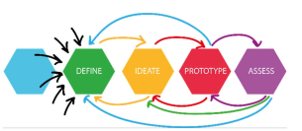
\includegraphics[width = 0.5\textwidth]{Revisao/VR Cabin/Process ilustration.png}
%    \caption{Simplified cabin design process \cite{moerland2021application}.}
%    \label{fig:simplified_cabin_process}
%\end{minipage}
%\hfil
%\begin{minipage}{\textwidth}
%    \centering
%    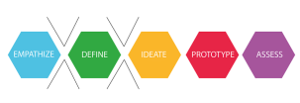
\includegraphics[width = 0.5\textwidth]{Revisao/VR Cabin/Design User involment.png}
%    \caption{Best moments for user involvement \cite{moerland2021application}.}
%    \label{fig:user_involvement}
%\end{minipage}
%\end{figure}

\begin{figure}[!htbp]
    \centering    
    \tikzstyle{hexag} = [regular polygon, regular polygon sides=6, minimum size = 3cm, inner sep = 0cm, xshift = 1.5cm]
    \tikzstyle{hexagText} = [text = white, xshift = 1.5cm]
    \tikzstyle{legenda} = [fill = white, line width = 0.25mm]
    \tikzstyle{--} = [line width = 0.25mm]
    
    \tikzstyle{arrow} = [rounded corners, line width = 1mm, -to]
    \tikzstyle{arrow_blue} = [cor5, arrow]
    
    \resizebox{\linewidth}{!}{
    \begin{tikzpicture}[node distance=1.75cm]
        \centering    

        \node [hexag, draw = cor1, fill = cor1] (emphatize) {};
        \node [hexagText] (emphatizeText) {};
        
        \node [hexag, draw = cor2, fill = cor2, right of = emphatize] (define) {};
        \node [hexagText, right of = emphatize] (defineText) {DEFINE};
        
        \node(inicioFlecha1) [xshift = 3.75cm, yshift = 2.25cm] {};
        \node(fimFlecha1) [right of = emphatize, xshift = 1cm, yshift = 1.2cm] {};
        \node(inicioFlecha2) [xshift = 2.75cm, yshift = 1.5cm] {};
        \node(fimFlecha2) [right of = emphatize, xshift = 0.5cm, yshift = 0.8cm] {};
        \node(inicioFlecha3) [xshift = 1.7cm, yshift = 0.8cm] {};
        \node(fimFlecha3) [right of = emphatize, xshift = 0.25cm, yshift = 0.4cm] {};
        \node(inicioFlecha4) [xshift = 2cm, yshift = -0.5cm] {};
        \node(fimFlecha4) [right of = emphatize, xshift = 0.15cm, yshift = 0cm] {};
        \node(inicioFlecha5) [xshift = 2.77cm, yshift = -1.6cm] {};
        \node(fimFlecha5) [right of = emphatize, xshift = 0.25cm, yshift = -0.5cm] {};
        \node(inicioFlecha6) [xshift = 3.4cm, yshift = -2.2cm] {};
        \node(fimFlecha6) [right of = emphatize, xshift = 0.8cm, yshift = -1.2cm] {};
        
        \draw[arrow] (inicioFlecha1) .. controls ++(0.3,-0.5) .. (fimFlecha1);
        \draw[arrow] (inicioFlecha2) .. controls ++(0.5,-0.15) .. (fimFlecha2);
        \draw[arrow] (inicioFlecha3) .. controls ++(0.75,0) .. (fimFlecha3);
        \draw[arrow] (inicioFlecha4) .. controls ++(0.5,0.25) .. (fimFlecha4);
        \draw[arrow] (inicioFlecha5) .. controls ++(0.25,0.5) .. (fimFlecha5);
        \draw[arrow] (inicioFlecha6) .. controls ++(0.25,0.5) .. (fimFlecha6);
        
        \node [hexag, draw = cor3, fill = cor3, right of = define] (ideate) {};
        \node [hexagText, right of = define] (ideateText) {IDEATE};
        
        \node(inicioDFlecha1) [above of = define, xshift = 0.25cm, yshift = -0.1cm] {};
        \node(fimDFlecha1) [above of = ideate, xshift = -0.25cm, yshift = -0.1cm] {};
        \node(inicioIFlecha1) [below of = ideate, xshift = -0.25cm, yshift = 0.1cm] {};
        \node(fimIFlecha1) [below of = define, xshift = 0.25cm, yshift = 0.1cm] {};
        
        \draw[arrow, draw = cor3] (inicioDFlecha1.south) .. controls ++(0.25,0.5) and ++(-0.75,0.5).. (fimDFlecha1.south);
        \draw[arrow, draw = cor3] (inicioIFlecha1.north) .. controls ++(-0.25,-0.5) and ++(0.75,-0.5).. (fimIFlecha1.north);
        
        \node [hexag, draw = cor4, fill = cor4, right of = ideate] (prototype) {};
        \node [hexagText, right of = ideate] (prototypeText) {PROTOTYPE};
        
        \node(inicioIFlecha2) [above of = ideate, xshift = 0.25cm, yshift = -0.2cm] {};
        \node(fimIFlecha2) [above of = prototype, xshift = -0.25cm, yshift = -0.2cm] {};
        \node(inicioPFlecha1) [below of = prototype, xshift = -0.25cm, yshift = 0.2cm] {};
        \node(fimPFlecha1) [below of = ideate, xshift = 0.25cm, yshift = 0.2cm] {};
        \node(inicioPFlecha2) [above of = prototype, xshift = 0.25cm, yshift = -0.2cm] {};
        \node(fimPFlecha2) [above of = define, xshift = -0.25cm, yshift = -0.2cm] {};
        
        \draw[arrow, draw = cor4] (inicioIFlecha2.center) .. controls ++(0.25,0.5) and ++(-0.75,0.5).. (fimIFlecha2.east);
        \draw[arrow, draw = cor4] (inicioPFlecha1.east) .. controls ++(-0.25,-0.5) and ++(0.75,-0.5).. (fimPFlecha1.center);
        \draw[arrow, draw = cor1] (inicioPFlecha2.west) .. controls ++(-1,1.75) and ++(1.2,1.5).. (fimPFlecha2);
        
        
        \node [hexag, draw = cor5, fill = cor5, right of = prototype] (assess) {};
        
        \node(inicioPFlecha3) [above of = prototype, xshift = 0.25cm, yshift = -0.2cm] {};
        \node(fimPFlecha3) [above of = assess, xshift = -0.25cm, yshift = -0.2cm] {};
        \node(inicioAFlecha1) [below of = assess, xshift = -0.25cm, yshift = 0.2cm] {};
        \node(fimAFlecha1) [below of = prototype, xshift = 0.25cm, yshift = 0.2cm] {};
        \node(inicioAFlecha2) [below of = assess, xshift = 0cm, yshift = 0.2cm] {};
        \node(fimAFlecha2) [below of = ideate, xshift = -0.25cm, yshift = 0.1cm] {};
        \node(inicioAFlecha3) [below of = assess, xshift = 0.25cm, yshift = 0.2cm] {};
        \node(fimAFlecha3) [below of = define, xshift = -0.25cm, yshift = 0.1cm] {};
        
        \draw[arrow, draw = cor5] (inicioPFlecha3.center) .. controls ++(0.5,1) and ++(-0.75,1).. (fimPFlecha3.center);
        \draw[arrow, draw = cor5] (inicioAFlecha1.center) .. controls ++(-0.25,-0.5) and ++(0.75,-1).. (fimAFlecha1.west);
        \draw[arrow, draw = cor2] (inicioAFlecha2.center) .. controls ++(-0.25,-1.25) and ++(0.75,-1).. (fimAFlecha2.south east);
        \draw[arrow, draw = cor1] (inicioAFlecha3.center) .. controls ++(-0.25,-1.75) and ++(1.2,-1.5).. (fimAFlecha3.north);
        
        \node [hexagText, right of = prototype] (assessText) {ASSESS};
        

        
        
    \end{tikzpicture}
    }
    \caption{Simplified cabin design process (Adapted from \citeonline{moerland2021application}).}
    \label{fig:simplified_cabin_process}
\end{figure}
\begin{figure}[!htbp]
    \centering    
    \tikzstyle{hexag} = [regular polygon, regular polygon sides=6, minimum size = 3cm, inner sep = 0cm, xshift = 1.5cm]
    \tikzstyle{hexagText} = [text = white, xshift = 1.5cm]
    \tikzstyle{legenda} = [fill = white, line width = 0.25mm]
    \tikzstyle{--} = [line width = 0.25mm]
    
    \resizebox{\linewidth}{!}{
    \begin{tikzpicture}[node distance=1.75cm]
        \centering    

        \node [hexag, draw = cor1, fill = cor1] {};
        \node [hexagText] (emphatize) {EMPHATIZE};
        %\node [regular polygon, regular polygon sides=6, text = white, draw = cor1, minimum size = 5cm, fill = cor1] (emphatize) {EMPHATIZE};
        \node [hexag, draw = cor2, fill = cor2, right of = emphatize] (define) {};
        \node [hexagText, right of = emphatize] (defineText) {DEFINE};
        %\node [regular polygon, regular polygon sides=6, text = white, draw = cor2, minimum size = 5cm, fill = cor2, right of = emphatize] (define) {DEFINE};
        \node [hexag, draw = cor3, fill = cor3, right of = define] (ideate) {};
        \node [hexagText, right of = define] (ideateText) {IDEATE};
        %\node [regular polygon, regular polygon sides=6, text = white, draw = cor3, minimum size = 5cm, fill = cor3, right of = define] (ideate) {IDEATE};
        \node [hexag, draw = cor4, fill = cor4, right of = ideate] (prototype) {};
        \node [hexagText, right of = ideate] (prototypeText) {PROTOTYPE};
        %\node [regular polygon, regular polygon sides=6, text = white, draw = cor4, minimum size = 5cm, fill = cor4, right of = ideate] (prototype) {PROTOTYPE};
        \node [hexag, draw = cor5, fill = cor5, right of = prototype] (assess) {};
        \node [hexagText, right of = prototype] (assessText) {ASSESS};
        %\node [regular polygon, regular polygon sides=6, text = white, draw = cor5, minimum size = 5cm, fill = cor5, right of = prototype] (assess) {ASSESS};

        \node(insertNorth1) [right of = emphatize, xshift = -0.125cm, yshift = 0.25cm] {};
        \node(insertNorthWest1) [above of = insertNorth1, left of = insertNorth1, xshift = 0.75cm] {};
        \node(insertNorthEast1) [above of = insertNorth1, right of = insertNorth1, xshift = -0.75cm] {};
        \draw[--] (insertNorthWest1.center) to (insertNorth1.center) to (insertNorthEast1.center);
        
        \node(insertSouth1) [right of = emphatize, xshift = -0.125cm, yshift = -0.25cm] {};
        \node(insertSouthWest1) [below of = insertSouth1, left of = insertSouth1, xshift = 0.75cm] {};
        \node(insertSouthEast1) [below of = insertSouth1, right of = insertSouth1, xshift = -0.75cm] {};
        \draw[--] (insertSouthWest1.center) to (insertSouth1.center) to (insertSouthEast1.center);
        
        \node(insertNorth2) [right of = define, xshift = -0.125cm, yshift = 0.25cm] {};
        \node(insertNorthWest2) [above of = insertNorth2, left of = insertNorth2, xshift = 0.75cm] {};
        \node(insertNorthEast2) [above of = insertNorth2, right of = insertNorth2, xshift = -0.75cm] {};
        \draw[--] (insertNorthWest2.center) to (insertNorth2.center) to (insertNorthEast2.center);
        
        \node(insertSouth2) [right of = define, xshift = -0.125cm, yshift = -0.25cm] {};
        \node(insertSouthWest2) [below of = insertSouth2, left of = insertSouth2, xshift = 0.75cm] {};
        \node(insertSouthEast2) [below of = insertSouth2, right of = insertSouth2, xshift = -0.75cm] {};
        \draw[--] (insertSouthWest2.center) to (insertSouth2.center) to (insertSouthEast2.center);


    \end{tikzpicture}
    }
    \caption{Best moments for user involvement \cite{moerland2021application}.}
    \label{fig:user_involvement}
\end{figure}


\citeauthor{moerland2021application} are inside the German Aerospace Center (DLR, \textit{Deutsch Zentrum für Luft- Raumfahrt}) and decided to study a new procedure that could bring the involvement from the final users in the design process. This procedure is based on co-design, where the users can influence the product's development from the beginning until the end. The Figure \ref{fig:user_involvement} shows the best moments to bring the users to the process. But for the involvement to happen, a communication channel needed to be established. The authors choose to use \textit{Reality Works} and test on a DLR's inside project. This project's goal was to design a new cabin that would be incorporated in a large workflow, but the design process was to be completely made in an digital environment. This was the perfect test case for the VR use in the cabin's design procedure.

A pilot use case was made with the members from this project. Three different designers (two with around 5 years of experience and other more than 35 years of experience) initiated a cabin design. 
The Figures \ref{fig:cabin_sketch} and \ref{fig:cabin_3d_model} show the results using the traditional method. The sketch can only present a glance of what the cabin will be. The 3D model has more details, but any change on this representation needs a new rendering session and this can take hours, or even days, to be made.

\begin{figure}[h]
\centering
\begin{minipage}{.45\textwidth}
    \centering
    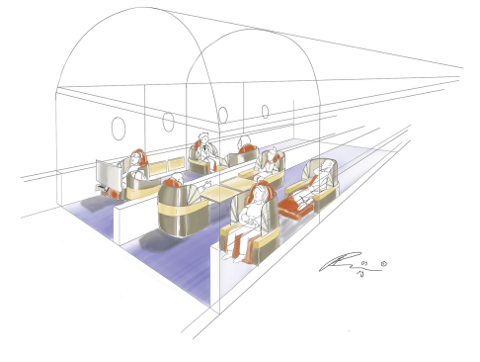
\includegraphics[width = \linewidth]{Revisao/VR Cabin/Sketch.png}
    \vspace{0.4cm}
    \caption{Cabin sketch made with Adobe Photoshop \cite{moerland2021application}.}
    \label{fig:cabin_sketch}
\end{minipage}
\hfil
\begin{minipage}{.45\textwidth}
    \centering
    \includegraphics[width = \linewidth]{Revisao/VR Cabin/3D Model.png}
    \caption{Cabin 3D model made with Rhyno \cite{moerland2021application}.}
    \label{fig:cabin_3d_model}
\end{minipage}
\end{figure}

The Figures \ref{fig:vr_sketch} and \ref{fig:vr_3d_model} show the same representation but made in a VR environment. The sketch was made inside the aircraft cabin and this could have been done with a client or a stakeholder and they could also draw and give their opinions from the beginning. The 3D models can be imported to increase the sketch's level of detail.

\begin{figure}[h]
\centering
\begin{minipage}{.45\textwidth}
    \centering
    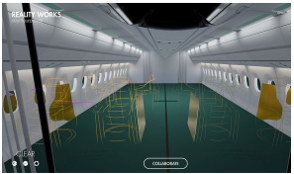
\includegraphics[width = \linewidth]{Revisao/VR Cabin/VR sketch.png}
    \caption{VR navigation with sketching \cite{moerland2021application}.}
    \label{fig:vr_sketch}
\end{minipage}
\hfil
\begin{minipage}{.45\textwidth}
    \centering
    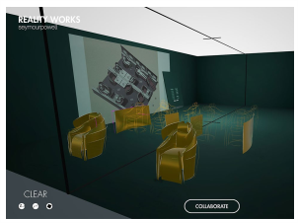
\includegraphics[width = \linewidth]{Revisao/VR Cabin/VR 3D Model.png}
    \caption{VR navigation with imported 3D models \cite{moerland2021application}.}
    \label{fig:vr_3d_model}
\end{minipage}
\end{figure}

This case was well received by the design team and they chosen to continue to use the VR tool. The benefits disadvantages pointed by \citeauthor{moerland2021application} are listed in the Table \ref{tab:benefits_disvantages_vr_cabin}. The VR definitely helps to brings the clients closer to the design team, allows to draw quick sketches in brainstorming gatherings and has a steep learning curve for the designers. On the other hand, is its a high cost tool, the use during a long time can cause nausea and maybe other health implications and, even though the learning curve is steep, there is still a learning curve and the user needs to get used with the exposure to others that can see the user from outside the virtual environment (some find this situation uncomfortable).

\begin{table}[h]
    \centering
    \caption{The benefits and disadvantages noted by the authors \citeauthor{moerland2021application}.}
    \label{tab:benefits_disvantages_vr_cabin}
    \begin{tabular}{|l|l|}
        \hline
        \textbf{Benefits}                         & \textbf{Disadvantages}                                  \\ \hline
        Bottleneck at early concept design stages & High cost                                               \\ \hline
        Quick sketchs during brainstorming        & Nausea and other health implacations                    \\ \hline
        Steep learning curve                      & \begin{tabular}[c]{@{}l@{}}There is a learning and personal\\ adaptation to exposure\end{tabular} \\ \hline
    \end{tabular}
\end{table}

The current master's thesis isn't about designing or aicraft cabin's, but this research shows that VR is being studied to be implemented inside industries. The current research could be done by any product industry that wanted to create a test environment for their clients in order to increase the user's approval or to bring other teams close to reduce the full design time.